%----------------------------------------------------------------
%
%  File    :  vpn_learning.tex
%
%  Author  :  Keith Andrews, IICM, TU Graz, Austria
% 
%  Created :  22 Feb 96
% 
%  Changed :  19 Feb 2004
% 
%----------------------------------------------------------------

\chapter{Learning}

\label{chap:Learning}

% Setup
\section{Environment Setup} \label{sec:learnenv}
% describe VMs, IPsec server software, configuration etc
We developed and tested our custom mapper using two VirtualBox 6.1 \ac{vm}s running standard Ubuntu 22.04 LTS distributions. Both VMs were allotted 4GB of memory and one CPU core. All communication took place in an isolated virtual network to eliminate possible external influences. During learning, all power saving options and similar potential causes of disruptions were disabled. For larger learning attempts, the \ac{ipsec} server was restarted before each attempt to ensure identical conditions. We designated one \ac{vm} as the initiator and one as the responder to create a typical client-server setup. The used Strongswan config files can be found in Appendix TODO. The open source \ac{ipsec} implementation Strongswan\footnote{https://www.strongswan.org/} was installed on the responder \ac{vm} and set to listen for incoming connections from the initiator \ac{vm}. We used the Strongswan version US.9.5/K5.15.0-25-generic, installed using the default Ubuntu package manager, apt. The Strongswan server was configured to use pre-shared keys for authentication and default recommended security settings. Additionally, it was configured to allow unencrypted notification messages, which we used to reset the connection during the learning process. For learning, we used the Python library \textsc{AALpy}\footnote{https://github.com/DES-Lab/AALpy} version 1.2.9 in conjunction with the packet manipulation library Scapy\footnote{https://scapy.net/}, version 2.4.5. Significant effort was put into expanding the \ac{isakmp} Scapy module to support all packets required for \ac{ipsec} as the module lacked many features out-of-the-box. The provided Python script, \emph{IPSEC\_IKEv1\_SUL} demonstrates how we use the \textsc{AALpy} in conjunction with our custom mapper to communicate with and learn the model of an \ac{ipsec} server.

\begin{figure}
	\centering
	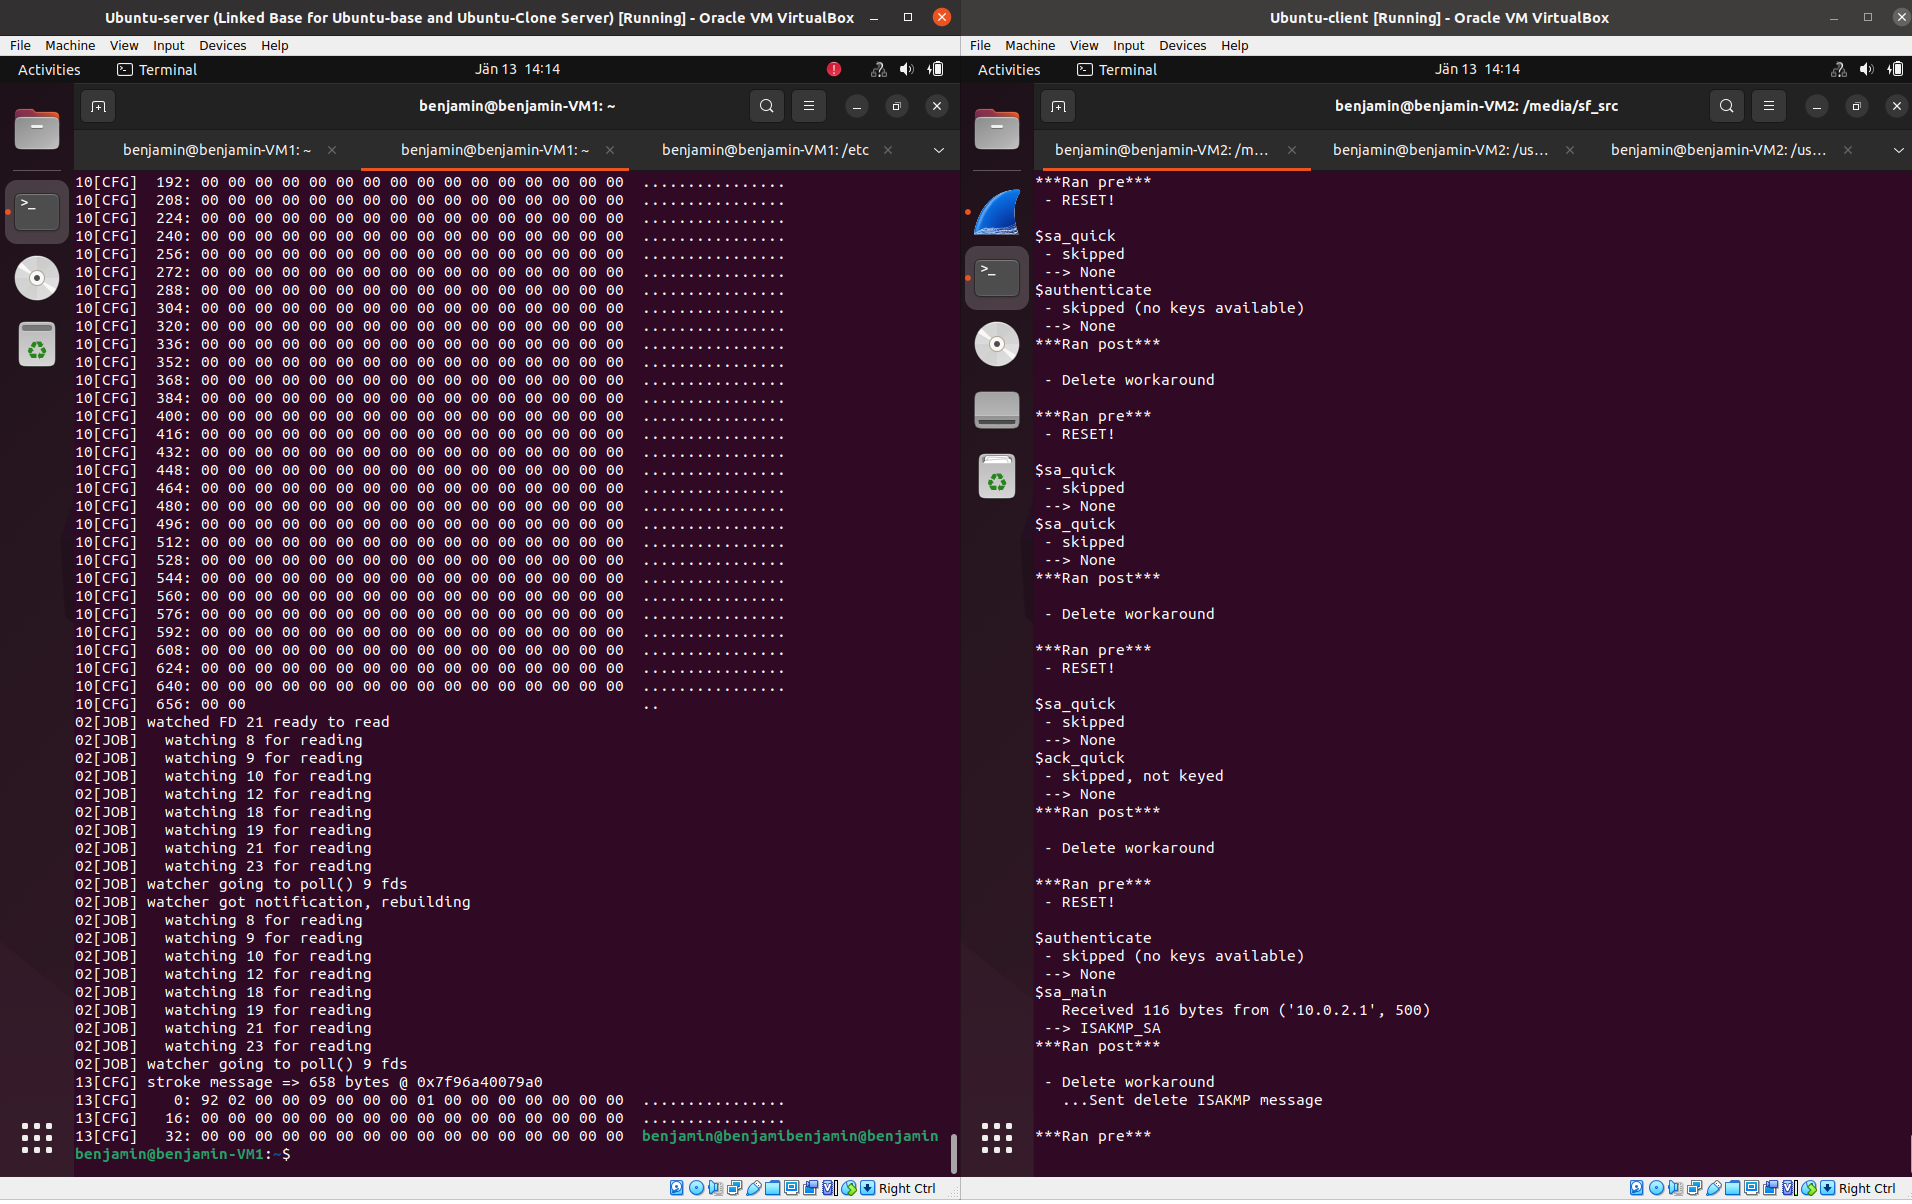
\includegraphics[width=\linewidth]{images/VM_setup}
	\caption{Learning setup, server left, learner right.}
	\label{fig:vmsetup}
\end{figure}

% non-eterminism fixes
\section{Combating Non-determinism} \label{subsec:nondet}
Despite all the precautions detailed in Section~\ref{sec:learnenv}, the \ac{ipsec} server still exhibited non-deterministic behavior, resulting in variance among the learned automata. While the majority of learned models were identical, the rest were significantly different, as can be seen when comparing Figure \ref{fig:nofilterb} to the more common ones shown in Chapter \ref{chap:Evaluation}. To help decrease the remaining non-deterministic behavior, timeouts were added to all requests in order to give the server more time to correctly work through all incoming requests. This measure helped further decrease the amount of outlying automata learned, however it did not fully fix the issue. Examination of the outliers led to the discovery that all outlying behavior was concentrated around so-called retransmissions. Essentially, the \ac{ike} specification allows for previous messages to be retransmitted if deemed useful. A possible trigger could be the final message of an \ac{ike} exchange being skipped / lost. For example, if instead of an \emph{AUTH} message, the server receives a phase two \emph{IPSEC SA} message, the server would not know if it missed a message or if their was an error on the other parties side. According to the \ac{isakmp} specification in RFC 2408~\parencite{rfc2408}, the handling of this situation is unspecified, however two possible methods are proposed. Firstly, if the \emph{IPSEC SA} message can be verified somehow to be correct, the server may ignore the missing message and continue as is. Secondly, the server could retransmit the message prior to the missing one to force the other party to respond in kind. Strongswan appears to implement these retransmissions and due to internal timeouts of connections, seem to trigger in a not-quite-deterministic fashion. These retransmissions also explain the strange transitions seen in phase two of Figure \ref{fig:nofilterb}. 

\begin{figure}[h]
	\centering
	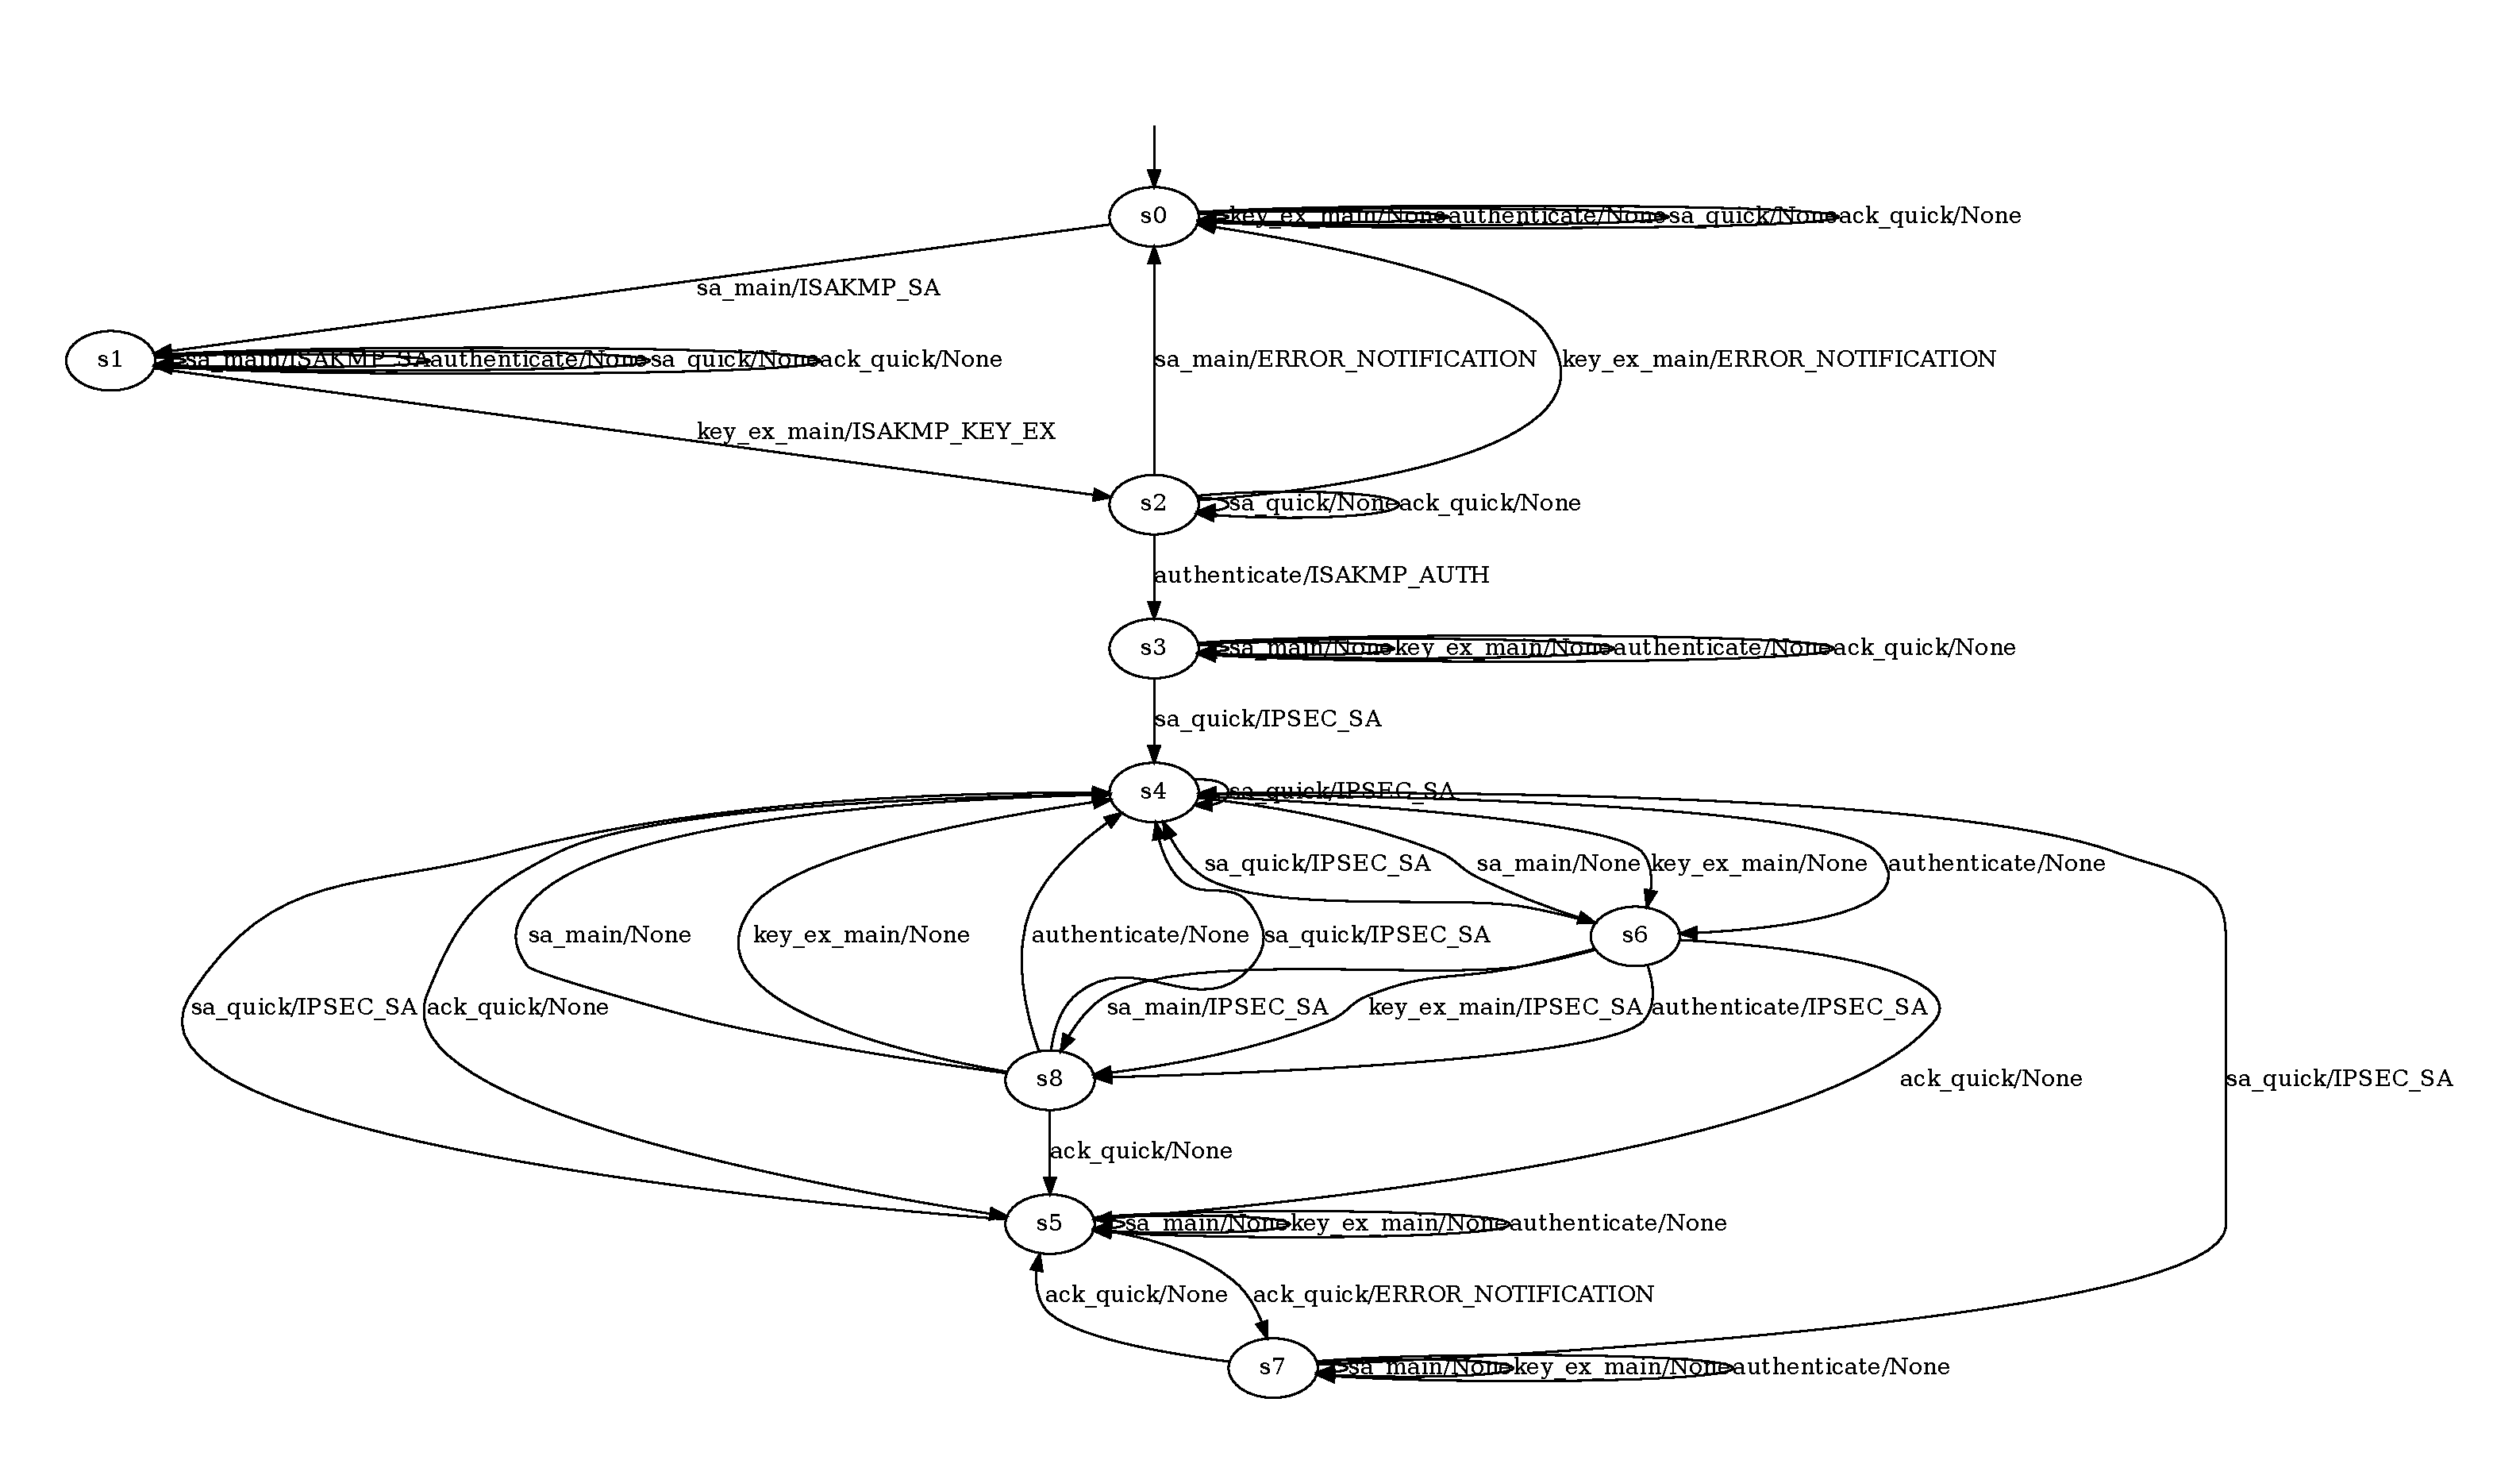
\includegraphics[width=0.7\linewidth]{images/models/NoFilterB}
	\caption{An example variant learned model.}
	\label{fig:nofilterb}
\end{figure}

While interesting for fingerprinting, we wanted a deterministic automaton as a base case for automata-based fuzzing, so we implemented checks in our mapper to allow the ignoring of retransmissions. The retransmission-filtering can be easily enabled or disabled through a simple flag and works by checking the message ID of incoming server responses against a list of previous message IDs (excluding zero, as it is the default message ID for phase one). If a repeated message ID is found, it is flagged as a retransmission and depending on the current filtering rule, ignored. With this addition, the \ac{ipsec} server became 100\% deterministic, allowing the learning of a very clean automata, as shown in Figure \ref{fig:reference}. As an additional method of dealing with non-determinism but still keeping retransmissions, we can also catch non-determinism errors as they occur and repeat the offending query several times. If upon the first rerun the non-determinism does not occur again, we accept the existing value as the correct one and continue. If however, it persists for a set amount of repetitions with the same constant server response, we assume that the original saved response was incorrect and update it to the new one. With this non-determinism correcting added, the automata learning also works with no more non-determinism errors and the learned automata are consistent with one another.


% Basic Model-Learning workflow
\section{Learning Setup} \label{subsec:learningenv}% half - quarter page
We used the Python automata learning library \textsc{AALpy} to learn our automata. It boasts support for deterministic, non-deterministic and stochastic automata, with support for various formalisms for each automata type. We chose deterministic Mealy machines to describe the \ac{ipsec} server. However, learning automata with \textsc{AALpy} follows the same pattern, regardless of the type of automata.

\begin{figure}[h]
	\begin{tikzpicture} 
		\node (n1) [draw, minimum width=7em, minimum height=3.5em, align=left] at (0,1) {~Learning\\~Algorithm};
		\node (n2) [draw, minimum width=7em, minimum height=3.5em, align=left] at (4.4,1) {~Mapper};
		\node(n3) [draw, minimum width=7em, minimum height=3.5em,  align=left] at (8.8,1) {~Interface\\~(Initiator)};
		\node(n4) [draw, minimum width=7em, minimum height=3.5em,  align=left] at (13.2,1) {~SUL\\~(Responder)};
		\draw [->] ($(n1)+(3.5em,+0.5em)$) -> ($(n2)+(-3.5em,+0.5em)$) node[midway,above,align=center] {\scriptsize~Abstract\\\scriptsize~Input};
		\draw [->] ($(n2)+(-3.5em,-0.5em)$) -> ($(n1)+(3.5em,-0.5em)$) node[midway,below,align=center] {\scriptsize~Abstract\\\scriptsize~Output};
		
		\draw [->] ($(n2)+(3.5em,+0.5em)$) -> ($(n3)+(-3.5em,+0.5em)$) node[midway,above,align=center] {\scriptsize~Concrete\\\scriptsize~Input};
		\draw [->] ($(n3)+(-3.5em,-0.5em)$) -> ($(n2)+(3.5em,-0.5em)$) node[midway,below,align=center] {\scriptsize~Concrete\\\scriptsize~Output};
		
		\draw [<->] (n3) -> (n4) node[midway,above,align=center] {\scriptsize~UDP};
		
		
	\end{tikzpicture} 
	\caption{Automata Learning Setup}
	\label{fig:AALSetup}
\end{figure}

Figure \ref{fig:AALSetup} gives an overview of the learning process, adapted from Tappler et al.~\cite{tappler2017}. To begin, the learning algorithm sends abstract inputs chosen from the input alphabet to the mapper class, which converts it to concrete inputs. The concrete inputs are then sent to the \ac{sul}, by means of a communication interface. In our case, the mapper class comprises the major portion of our work and converts the abstract words into actual \ac{ipsec} packets that can be sent to the \ac{sul} Strongswan server via UDP packets. This separation between abstract and concrete in/outputs allows for easy future modifications to the message implementations, including fuzzing support, as well as increasing the readability of our code.

To begin learning an automaton with \textsc{AALpy}, we must first choose a suitable input alphabet encompassing the language known by the server, as well as the learning algorithm to be used. Our chosen input alphabet consists of the initiator-to-responder messages shown in Figure \ref{fig:IKEv1}. We use both the $L^*$ and $KV$ algorithms for learning with a state prefix equivalence oracle that provides state-coverage by means of random walks started from each state. The equivalence oracle is used by the chosen learning algorithm to test for conformance between the current hypothesis and the \ac{sul}, giving either a counterexample on failure, or confirmation that we have learned the \ac{sul}. This corresponds to an equivalence query. We also enabled several optional \textsc{AALpy} features including caching and non-determinism checks to improve the learning process. An overview of relevant code can be seen in Listing \ref{lst:eqcode}. Line three shows the used input alphabet, line four the used equivalence oracle and line 5 the used learning algorithm. Both the equivalence oracle and learning algorithm take the input alphabet and an object representing the \ac{sul} as parameters, were the \ac{sul} is defined as shown below in \ref{lst:membercode}. The equivalence oracle is then also passed as a parameter to the the learning algorithm which also has a few additional optional parameters specifying the type of automaton to learn and enabling non-determinism checking and caching.

\begin{lstlisting}[float=h, caption=Equivalence Query code, label=lst:eqcode, language=python]
	# Code example detailing AAL with AALpy
	
	input_al = ['sa_main', 'key_ex_main', 'authenticate', 'sa_quick', 'ack_quick']
	eq_oracle = StatePrefixEqOracle(input_al, sul, walks_per_state=10, walk_len=10)
	learned_ipsec = run_Lstar(input_al, sul, eq_oracle=eq_oracle, automaton_type='mealy', cache_and_non_det_check=True)
	
\end{lstlisting}

To learn the target server, we defined a \emph{step} method and \emph{reset} functionality as can be seen in Listing \ref{lst:membercode}. We use \emph{step}, seen in line three, to execute one input action from the current query and \emph{reset}, lines eight through 12, to revert the \ac{sul} to an initial clean state. Used in combination, they correspond to membership queries, were \emph{step} is used to query the \ac{sul} with one letter of the input alphabet and \emph{reset} ensures identical starting conditions for each full query. \emph{pre} is called before each membership query and \emph{post} afterwards. The abstract input chosen from the input alphabet is passed on to the mapper class for further processing. We can see in line four, that a function, corresponding to the input, is called in the mapper class and the return value is passed on to the learning algorithm. \\

\begin{lstlisting}[float=h, caption=Membership Query code, label=lst:membercode, language=python]
	# code excerpt from IPSEC_IKEv1_SUL.py
	
	def step(self, letter):
		func = getattr(self.ipsec, letter)
		ret = func()
		return ret
	
	def pre(self):
		self.ipsec.reset()
		
	def post(self):
		self.ipsec.delete()
\end{lstlisting}

Our mapper class implements methods for each communication step in a typical \ac{ipsec}-\ac{ike}v1 exchange, as described in Section \ref{chap:Preliminaries}. This includes the \emph{ISAKMP SA}, \emph{KE}, \emph{AUTH}, \emph{IPSEC SA}, \emph{ACK} and \emph{DELETE} messages. The \emph{DELETE} message is special in that it actually sends two packets which is required to delete all existing connections to the Strongswan server. Also its behavior is highly dependent on the current state of the protocol. For these two reasons, it was mostly left out of the learning process. Furthermore, the mapper class contains a variety of helper functions used to handle the decryption and encryption of packets as well as parse received informational messages. To illustrate our mapper functions, (simplified) excerpts from \emph{ISAKMP SA} function are shown in Listing \ref{lst:mapper1}. It shows how a Scapy packet is constructed out of many different individually configurable layers and fields, allowing for a high degree of flexibility and customizability. We can see in line five, how an \ac{isakmp} transform is created, encompassing various security parameters. This is packed into a \ac{isakmp} proposal packet first and then the resulting packet is packet into an \ac{isakmp} \ac{sa} packet in line six. The \ac{sa} packet is appended to a generic top level \ac{isakmp} packet in line eight. In line nine we then send the \ac{isakmp} packet to the \ac{sul} and receive its response (if any) back, already converted into a matching Scapy object. The response then undergoes a retransmission check and is then parsed and relevant data is used to update local values in lines 11 through 16.

\begin{lstlisting}[float=h, caption=Excerpt of SA Main Mapper code, label=lst:mapper1, language=python]
	# code excerpt from IPSEC_MAPPER.py
	
	def sa_main(self, ...):
		...
		tf = [('Encryption', 'AES-CBC'), ('KeyLength', 256), ('Hash', 'SHA'), ('GroupDesc', '1024MODPgr'), ('Authentication', 'PSK'), ('LifeDuration', 28800)]
		sa_body_init = ISAKMP_payload_SA(prop=ISAKMP_payload_Proposal(trans_nb=1, trans=ISAKMP_payload_Transform(num=1, transforms=tf)))
		
		policy_neg = ISAKMP(init_cookie=cookie_i, next_payload=1, exch_type=2)/sa_body_init
		resp = self._conn.send_recv_data(policy_neg)
		
		if (ret := self.get_retransmission(resp)): 
			# retransmission handling
			...
		
		# Response handling (checks response code, decrypts if necessary, updates relevant local values)
		...
\end{lstlisting}

The \ac{ipsec} packets generated by the mapper class are passed on to our communication class, which acts as an interface for the \ac{sul} and handles all incoming and outgoing UDP communication. Additionally, it parses responses from the \ac{sul} into valid Scapy packets and passes them on to the mapper class. The mapper class then parses the received Scapy packets and returns an abstract output code representing the received data to the learning algorithm. This code corresponds to the type of received message, or in the case of an error response (informational message), the error type. For fuzzing purposes, several common error types were grouped together into categories and the error category was used as the return value. Finally, the abstract error codes are returned to the learning algorithm which uses it update its internal data structures and improve its understanding of the \ac{sul}. \\


\section{Design Decisions and Problems} \label{subsec:design}
% Design details advantages and disadvantages --> problems and solutions (2-3p)

As messages will be sent in random order during learning, we require a robust framework that correctly handles en/decryption of messages. For key management, we simply store the current base-keys but keep track of \ac{iv}s on a per \ac{mid} basis. Additionally, we keep track of the M-IDs of server responses to detect and handle retransmissions of old messages. Each request, we store the response for use in the next message and update affected key material as needed. Most notably, the \ac{iv}s are updated almost every request and differ between M-IDs. Informational requests also handle their \ac{iv}s separately. For each request that we send, if available, we try to parse the response, decrypting it if necessary and resetting or adjusting our internal variables as required to match the server. To keep track of all the different \ac{mid}s, we use a Python dictionary to map \ac{mid} to relevant keying and \ac{iv} information. Usually, \ac{iv}s are updated to the last encrypted block of the most recently sent or received message, though this behavior varies slightly between phases and for informational messages. Keeping track of \ac{iv}s is required to continuously be able to parse encrypted server responses and extract meaningful information. 

To ensure that we receive all responses, we add a timed wait for each server response, after which a None response is logged. In the case of no response, we can directly return None and need no further handling. Otherwise, we check the response \ac{mid} against our list of previous \ac{mid}s to detect retransmissions and then depending on the configured retransmission-handling rule, either ignore or use the corresponding previous response. To save some time when not ignoring retransmissions, we keep a dictionary mapping \ac{mid}s to their parsed response codes, allowing us to skip the parsing stage fro retransmitted messages. If no retransmission is detected, we check that the message type matches the expected one and if so, parse the message further to update local values and extract a response code. If the message type does not match, it is usually an informational message, indicating some sort of error. In that case we decrypt the message using the corresponding parameters (as they are calculated and saved differently for informational messages), and return a code indicating the error being reported. Finally we catch and log unimplemented message types, but this case should not occur unless fuzzing breaks something.


We use the Python library Scapy to construct \ac{isakmp} packets as required by the \ac{ike}v1 protocol. More exactly, we use the \ac{isakmp} package that defines a generic top-level \ac{isakmp} package as well as several more specific payloads that it can contain. Parsing was made more difficult by the fact that Scapy does not support / implement all the packets required by \ac{ipsec}-\ac{ike}v1. To solve this problem, we implemented all missing packets in the Scapy \ac{isakmp} class and used this modified version. Specifically, we added support for \ac{isakmp} Informational packets, including resolving all commonly supported error codes, \ac{isakmp} Delete packets, NAT-D, additional SA attributes for \ac{isakmp} and ESP. Additionally we improved the \ac{isakmp} Transform, Proposal and ID packets. 

In addition to all the \ac{isakmp} packets, Automata learning requires a \ac{sul} reset method to be able to return to an initial starting point after each query. We implement this using a combination of the \ac{isakmp} \emph{DELETE} request and general \ac{isakmp} informational error messages. While \emph{DELETE} works for established connections in phase two of \ac{ike}, we require informational error messages to trigger a reset in phase one, as delete does not work here sufficiently. Implementation was hindered at times by unclear RFC-specifications, but this was overcome by manually comparing packet dumps and Strongswan logs to fix encryption errors.\\

Each concrete mapping function in our mapper class can be run normally, with an injected error or with arbitrary values for the respective fields of the resulting packet. This allows us to learn different variations of the \ac{ipsec} server. For example, our mapper class allows us to very easily switch between learning the server model when presented with valid inputs, and the model of the server when introduced to invalid, malformed messages in combination with valid ones. Additionally, this design of the mapper functions will make fuzz testing specific protocol messages quite simple. The model of the server presented with malformed inputs will serve as the basis for future model based fuzz testing and can be seen in Chapter~\ref{chap:Evaluation}.

Since bugfixes and new features required a lot of testing and automata learning can be a very time-intensive process, we implemented several performance improvements to speed up the learning process. First we reduced the timeouts down to a minimum amount needed to still get deterministic results. Next we categorized the server informational responses according to their severity and impact and then grouped the most common ones together under the same abstract response code. This decreased the amount of states that had to be learned while at the cost of some information, but since any deviations or non-deterministic behavior would have been caught by the framework, we are confident that no important information was lost. Finally we switched out the $L^*$ learning algorithm for $KV$, as $KV$ can be more performative for learning environments where membership queries are expensive operations. As \ac{ike}v1 is a networks protocol with quite a bit of communication in each phase and we additionally have to implement small timeouts to wait for the server, each individual membership query can take several seconds. With hundreds of membership queries required to learn the \ac{ipsec} server, this results in a lot of time spent running the algorithm. Consequently, any decrease to the amount of membership queries should, in theory, lead to an overall decrease in runtime. Since \textsc{AALpy} supports the $KV$, switching between the two learning algorithms is as easy as setting a simple flag as shown in line three of Listing \ref{lst:newalg} below. The $KV$ algorithm, as expected, required less membership queries to learn the \ac{sul} and consequently significantly improved the speed at which models could be learned. The detailed comparison of runtime statistics between $L^*$ and $KV$ can be found in Chapter \ref{chap:Evaluation}.

\begin{lstlisting}[float=ht, caption=Switching Learning Algorithms, label=lst:newalg, language=python]
	# code excerpt from IPSEC_IKEv1_SUL.py
	
	if kv:
		learned_ipsec, info = run_KV(input_al, sul, eq_oracle, automaton_type='mealy', cex_processing='rs')
	else:
		learned_ipsec, info = run_Lstar(input_al, sul, eq_oracle=eq_oracle, automaton_type='mealy', cache_and_non_det_check=True)
\end{lstlisting}
